\subsubsection{Gestational Age of Babies in ACT}
Gestational age refers to the amount of time a fetus has spent in the womb, starting from the first day of the mother's last menstrual period. It is typically measured in weeks and is used to track fetal development and monitor the progress of pregnancy.

Babies born between 37 and 40 weeks are considered full-term and are generally at a lower risk for complications than those born earlier. These babies have had enough time to develop and mature in the womb, which can help ensure that they are able to breathe, eat, and maintain their body temperature after birth.

Babies born before 37 weeks are considered premature and may require special care and monitoring in a neonatal intensive care unit (NICU). Premature babies are at a higher risk for a range of complications, including respiratory distress syndrome, jaundice, and infections.

On the other hand, babies born after 40 weeks are considered post-term and may also be at a higher risk for complications, such as macrosomia (large birth weight), meconium aspiration syndrome, and fetal distress. In these cases, medical professionals may recommend inducing labor to ensure the health and safety of both the mother and the baby.

\begin{figure}
  \centering
  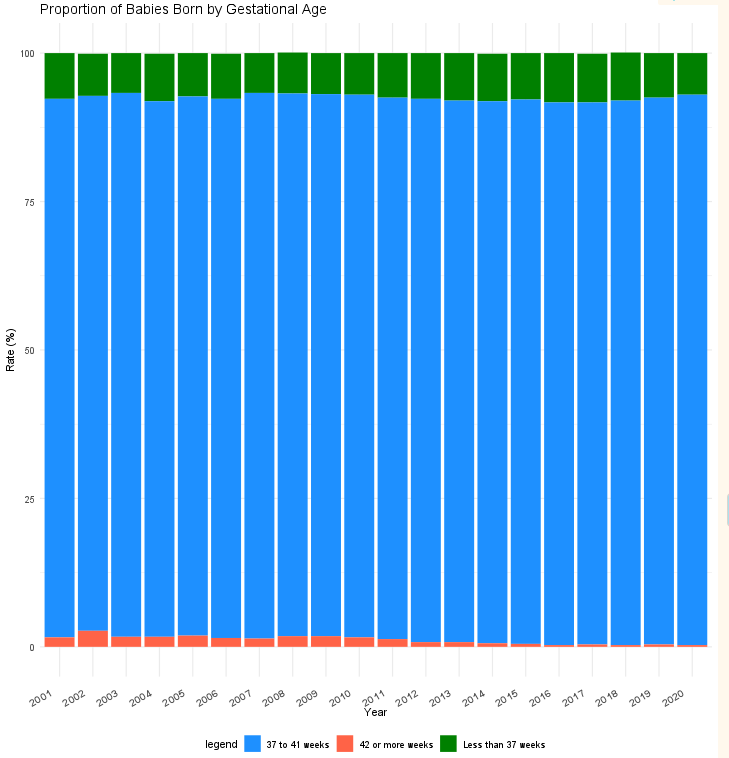
\includegraphics[width=0.8\textwidth]{subsections/baby_health/gestational_age_act.png}
  \caption{Gestational age of babies in ACT.}
  \label{fig:gest_act}
\end{figure}

In \textbf{Figure \ref{fig:gest_act}} we can see that the gestational age of babies has been really good which is over 90\%.